%%%%%%%%%%%%%%%%%%%%%%%%%%%%%%%%%%%%%%%%%
% Beamer Presentation
% LaTeX Template
% Version 1.0 (10/11/12)
%
% This template has been downloaded from:
% http://www.LaTeXTemplates.com
%
% License:
% CC BY-NC-SA 3.0 (http://creativecommons.org/licenses/by-nc-sa/3.0/)
%
%%%%%%%%%%%%%%%%%%%%%%%%%%%%%%%%%%%%%%%%%

\documentclass[t,usenames,dvipsnames]{beamer}
\mode<presentation> {
\usetheme{Boadilla}
\setbeamertemplate{navigation symbols}{} % To remove the navigation symbols from the bottom of all slides uncomment this line
}

\usepackage{graphicx} % Allows including images
\usepackage{booktabs} % Allows the use of \toprule, \midrule and \bottomrule in tables
\usepackage{amsmath}
\usepackage{amsthm}
\usepackage{cancel}
\usepackage{bussproofs}
\usepackage{proof}

\newcommand {\nconf}{\operatorname{neg}}

\title[space vs. width in resolution]
{Small space in resolution calculus implies small width
\texorpdfstring{\footnote{\tiny Filmus et al., From Small Space to Small Width in Resolution, ACM Trans.
Comput., 2015.}}}

\author{Narek Bojikian} % Your name
\institute[hu-berlin] % Your institution as it will appear on the bottom of every slide, may be shorthand to save space
{
Humboldt University of Berlin\\ % Your institution for the title page
\medskip
\textit{bojikian@informatik.hu-berlin.de} % Your email address
}
\date{10.07.2020} % Date, can be changed to a custom date

\begin{document}

\begin{frame}
\titlepage % Print the title page as the first slide
\end{frame}
\begin{frame} \frametitle{Introduction}
	\begin{itemize}[<+->]
		\item Literals, clauses, terms and normal forms.
			\begin{itemize}[<+->]
				\item Let $V = \{x, y, z\}$ be set of boolean-variables.
				\item Literals are negative and positive variables,
					\hspace{1cm} e.g. $x, \overline y,\dots$.
				\item A clause is a disjunction of literals,
					\hspace{1cm} e.g. $C = x \lor \overline y$.
				\item A term is conjunction literals,
					\hspace{1cm} e.g. $T = x \land \overline y$.
				\item A CNF formula is a conjunction of clauses.\\
					\hspace{1cm} e.g. $F := \{ \{x, y\}, \{\overline y, z\}\}$.
				\item A DNF
					\footnote{\uncover<8->{We write Clauses, terms and normal forms
					as sets and differentiate between them from the context,
					e.g. we write the clause $(x \lor \overline y)$ as $\{x,
					\overline y\}$}.} formula is a disjunction of terms.\\
				\item[]
				\item[--] A clause $C$ subsumes another clause $C'$ if $C \subseteq C'$.
				\item[--] We denote the empty clause by $\bot$ and the empty term
					by $\emptyset$.
				\item[--] A k-CNF (k-DNF) Formula is a CNF (DNF) formula where each
					clause (term) has at most $k$ literals.
			\end{itemize}
		\item Assignments.
			\begin{itemize}
				\item Boolean functions $\alpha: V \rightarrow \{0, 1\}$.
				\item $\alpha$ ``staisfies'' a circuit $F$ ( i.e. $\alpha \models F$), if
					$\alpha(F) = 1$ 
			\end{itemize}
	\end{itemize}
	
\end{frame}
\begin{frame}\frametitle{Introduction (Cont.) - Resolution proof}
	\begin{itemize}[<+->]
		\item A resolution configuration is a set of clauses.
		\item A resolution refutation of a CNF formula.
		\item[]
	\end{itemize}
	\uncover<3->{ \vspace{-.5cm}\begin{block}{Resolution refutation}
		A resolution refutation of a CNF-Formula $F$ is a sequence of configuration
		$\mathbb{C}_0 \dots \mathbb{C}_{\tau}$ such that:
		\begin{itemize}[<+->]
			\item $\mathbb{C}_0 = \emptyset$.
			\item $\bot \in \mathbb{C}_{\tau}$.
			\item $\mathbb{C}_i$ results from $\mathbb{C}_{i-1}$ by one of the following
				rules:
				\begin{itemize}
					\item[--] Axiom download. $\mathbb{C}_i = \mathbb{C}_{i-1} \cup
						\{A\}$, where $A \in F$ and $ A \notin
						\mathbb{C}_{i-1}$.
					\item[--] Erasure. $\mathbb{C}_i = \mathbb{C}_{i-1} \setminus
						\{A\}$, where $A \in \mathbb{C}_{i-1}$.
					\item[--] Inference. $\mathbb{C}_i = \mathbb{C}_{i-1} \cup
						\{A\}$, where $A \notin \mathbb{C}_{i-1}$ inferred
						by one of the following rules (here $\alpha$ denote
						a literal and $G, H$ denote clauses.
						\begin{itemize}
							\item
				$\displaystyle \frac{\overline{\alpha} \lor G \quad \alpha \lor H}{G \lor H}$
							\item 
				$\displaystyle \frac{G}{G\lor H}$ for an any clause $H$.
						\end{itemize}
				\end{itemize}
		\end{itemize}
	\end{block}}
\end{frame}

\begin{frame}\frametitle{Complexity measure of a resolution proof}
	\begin{block}{Complexity measures of a refutation}
		Let $\pi$ be a resolution refutation of a CNF formula $F$. We define the
		following complexity terms of $\pi$:
		\begin{itemize}[<+->]
			\item Length $L(\pi)$: the number of axiom-download and
				inference steps in $\pi$.
			\item Clause space $Sp(\pi)$: the max. number of clauses in a
				configuration.
			\item Width $W(\pi)$: the size of the largest clause in $\pi$.
			\item Depth $D(\pi)$: the maximum length of a root-leaf path in the
				derivation tree (excluding erasure).
		\end{itemize}

		\pause%
		The length ($L(F \vdash \bot)$) of refuting $F$ is the minimum length of a
		refutation of $F$.
		
		\pause%
		In an analogous way we define the space $Sp(F \vdash \bot)$, the width $W(F
		\vdash \bot)$ and the depth $D(F \vdash \bot)$ of refuting $F$.
	\end{block}

	\pause
	\noindent \underline{Note.} A Configuration $\mathbb{C}_i$ at a step $i$ is the set of all
	clauses we derive up to the step $t$ that will be needed after the step $t$.
\end{frame}
\begin{frame}\frametitle{Example - Resolution refutation}
	$F = \{ \{a, b\}, \{\overline a\}, \{\overline b\}\}.$ \pause
	\begin{center}
	\begin{tabular}{p{.45\textwidth}|p{.45\textwidth}}
		Refutation  $(\pi)$ & Rule\\ 
		\midrule
		$\emptyset$ &\\
		$\{\{a, b\}\}$ & Axiom Download\\
		$\{\{a, b\}, \{\overline a\}\}$ & Axiom Download\\
		$\{\{a, b\}, \{\overline a\}, \{b\}\}$ & Inference\\
		$\{\{b\}\}$ & Erasure\\
		$\{\{b\}, \{\overline b\}\}$ & Axiom Download\\
		$\bot$& Inf.+Er.\\
	  \end{tabular}
	\end{center} \pause
	\begin{itemize}[<+->]
		\item $L(\pi) = 5$.
		\item $Sp(\pi) = 3$.
		\item $W(\pi) = 2$.
		\item $D(\pi) = 2$
	\end{itemize}
\end{frame}
\begin{frame}\frametitle{Space is a lower-bound on depth}
	\begin{block}{Proposition}
		For each derivation of depth at most $k$ there is a derivation of clause-space at
		most $k$.
	\end{block}
	\pause
	\begin{itemize}[<+->]
		\item Use the derivation tree to build a new derivation of bounded space.
		\item Recursively build each sub-tree with bounded space and remove all but the last
			clause.
	\end{itemize}
	\pause
	\noindent \textbf{\underline{Remark.}} Meanwhile the length has an exponential lower-bound,
	it is not hard to show that the clause-space, the width and the depth are bounded in a
	linear function in the number of the variables.
\end{frame}
\begin{frame}
	\frametitle{Space is as a lower-bonud for width}
	\begin{block} {Theorem~3.1 [cf. Atserias and Dalmau, 2008]}
		Let $F$ be a $k$-CNF formula and let $\pi:F\vdash \bot$ be a resolution refutation
		in clause space $Sp(\pi) = s$. Then, there is a resolution refutation $\pi'$ of $F$
		in width $W(\pi') \leq s + k - 3$.
	\end{block}
	Proof idea and example:

	\pause
	\only<2-5>{
		\begin{itemize}[<+->]
		\item  Negate each configuration in the refutation.
		\item  Rewrite resulting formulas as configurations.
		\item[--] Width is bounded by number of clauses in a configuration (space).
		\item The resulting sequence in \textbf{backward} order is (almost) a valid
			refutation.
	\end{itemize}}
	\only<6>{ $F = \{ \{a, b\}, \{\overline a\}, \{\overline b\}\}.$ \pause
	\begin{center}
	\begin{tabular}{p{.25\textwidth}|p{.2\textwidth}|p{.27\textwidth}}
		Refutation &  Negation & Neg. as a conf.\\ 
			\midrule
		$\emptyset$ & $\bot$ & $\bot$\\
		%
		$\{\{a, b\}\}$ &
		$\overline a \land \overline b$&
		$\{\{\overline a\}, \{\overline b\}\}$\\
		%
		$\{\{a, b\}, \{\overline a\}\}$&
		$(\overline a \land \overline b)\lor a$&
		$\{\cancel{\{\overline a, a\}}, \{\overline b, a\}\}$\\
		%
		$\{\{a, b\}, \{\overline a\}, \{b\}\}$& 
		$(\overline a \land \overline b) \lor a \lor \overline b$&
		$\{\cancel{\{\overline a, a, \overline b\}}, \{\overline b, a, \overline b\}\}$\\
		%
		$\{\{b\}\}$&
		$\overline b$&
		$\{\{\overline b\}\}$\\
		%
		$\{\{b\}, \{\overline b\}\}$&
		$\overline b \lor b$&
		$\{\cancel{\{\overline b, b\}}\} = \emptyset$\\
		%
		$\{\} = \bot$& $\emptyset$ & $\emptyset$\\
	\end{tabular}
	\end{center}}
\end{frame}

\begin{frame}\frametitle{Theorem~3.1 Proof sketch}
	\begin{block} {Negated configuration ($\nconf(\mathbb{C})$)}
		$\nconf(\mathbb{C})$ of a clause configuration $\mathbb{C}$ is recursively defined
		as follows:
		\vspace{-.3cm}
		\pause
		\begin{alignat*}{3}
			&\nconf(\emptyset) = \{\bot\}&&\\
			%
			\uncover<3->{
			&\nconf(\mathbb{C} \cup \{C\}) =&& \{\underbrace{D \lor \overline a | D \in
					\nconf(\mathbb{C}); a \in C \setminus D }_{(*)};\\
			& &&\underbrace{\not \exists B \in \nconf(\mathbb{C}) s.t. B \lor \overline
				a \varsubsetneq D \lor \overline a}_{(**)}\}.}
		\end{alignat*}
	\end{block}
	\pause 
	\pause
	\begin{itemize}[<+->]
		\item The part $(*)$ represents one clause of $\nconf(\mathbb{C})$ as seen in the
			previous example (due to distributivity of $\lor$).
		\item The part $(**)$ ensures the minimality (inclusion wise) of the clauses and
			hence no trivial or subsummed clauses are contained in $\nconf(\mathbb{C})$.
	\end{itemize}
\end{frame}

\begin{frame}\frametitle{Theorem~3.1. Proof sketch (Cont.)}
	\begin{block}{Observation~3.3.}
		The width of any clause in the negated configuration $\nconf(\mathbb{C})$ is at most
		$Sp(\mathbb{C}_t) = |\mathbb{C}|$.
	\end{block}
	\pause
	\only<2>{ \noindent Proof sketch. Each clause in $\mathbb{C}$ contributes at most one literals to
	each clause inthe negated configuration.\hfill $\square$}
	\pause
	\begin{block}{Proposition~3.4.}
		The negated configuration $\nconf(\mathbb{C})$ is the set of all minimal
		(nontrivial) clauses $C$ such that $\lnot C$ implies the configuration $\mathbb{C}$.
		That is,
		\vspace{-.3cm}
		$$\nconf(\mathbb{C}) = \{C|\lnot C \models \mathbb{C} \text{ and for every } C'
		\varsubsetneq C \text{ it holds that } \lnot C' \not \models \mathbb{C}.\}$$
	\end{block}
	\pause
	\only<4>{ \noindent Proof Idea. Let $\mathbb{D}$ be the set of minimal clauses whose complements imply
	$\mathbb{C}$. Show that for $C \in \nconf(\mathbb{C})$ there is a $C' \in \mathbb{D}$ such
	that $C' \subseteq C$ and vise versa. Since both sets contain only minimal clauses, the
	claim follows.}
	\pause
	\only<5->{ \begin{block}{Observatoin~3.5.}
		An assignment satisfies a clause configuration $\mathbb{C}$ if and only if it
		falsifies the negated clause configuration $\nconf(\mathbb{C})$. That is,
		$\mathbb{C}$ is logically equivalent to $\lnot \nconf(\mathbb{C})$.
	\end{block}}
\end{frame}
\begin{frame}\frametitle{Theorem 3.1. Proof sketch (Cont. 2)}
	\begin{block}{Lemma~3.6.}
		If $\mathbb{C} \models \mathbb{C}'$, then for every clause $C \in
		\nconf(\mathbb{C})$ there exists a clause $C' \in \nconf(\mathbb{C}')$ such that $C$
		is a weakening of $C'$.
	\end{block}
	\pause
	Remark. This ensures that erasure and inference do not increase the width over the maximum
	width of a clause in a refutation (i.e. at most $s$).
	\pause
	\begin{itemize}[<+->]
		\item Let $\pi = (\mathbb{C}_0, \mathbb{C}_1, \dots \mathbb{C}_{\tau})$.
		\item Let $\pi' = (\mathbb{D}_{\tau}, \dots, \mathbb{D}_0), \mathbb{D}_i =
			\nconf(\mathbb{C}_i)$.
		\item $\bot \in \mathbb{D}_0$ and $\mathbb{D}_{\tau} = \emptyset$.
		\item {\color{red}Assume} for now that $k \geq 3$.
		\item If $\mathbb{C}_{t-1} \models \mathbb{C}_{t}$ (Lemma~3.6.),
		\item[] \hspace{.5cm} $\implies$  $\mathbb{D}_{t-1}$ is a weakening of $\mathbb{D}_t$.
		\item Interesting case: $\mathbb{C}_{t-1} \not \models \mathbb{C}_{t}$
		\item[] \hspace{.5cm} ($\implies$ Axiom Download at step $t$).
	\end{itemize}
\end{frame}

\begin{frame}\frametitle{Theorem 3.1. Proof sketch (Cont. 3)}
	\begin{block}{Claim.}
		If $\mathbb{C}_t$ results from $\mathbb{C}_{t-1}$ through an axiom-download step, it
		follows that $W(\mathbb{D}_t \vdash \mathbb{D}_{t-1}) \leq s + k - 3$.
	\end{block}
	\pause
	\begin{minipage}[t]{0.6\linewidth}
	\begin{itemize}[<+->]
		\item Assume $Sp(\mathbb{C}_{t-1}) \leq s - 2$. \textbf{(Why?)}
		\item Let $\mathbb{C}_t = \mathbb{C}_{t-1} \cup A$,\\
			$A = \{a_1, \dots a_{\ell}\} \in F, \ell \leq k$.
		\item Choose $C \in \mathbb{D}_{t-1} \setminus \mathbb{D}_t$, (Obs. 3.3).
		\item[] $W(C) \leq Sp(\mathbb{C}_{t-1}) \leq s-2$ 
		\item First download $A$ then derive $C$\\
			from $\mathbb{D}_{t} \cup \{A\}$ as follows.
		\item Note that each $C \lor \overline a_i$ is\\
			in or a weakening of a clause in $\mathbb{C}_t$.
	\end{itemize}
	\end{minipage}%
	\hfill%
	\begin{minipage}[t]{0.39\linewidth}
	\pause
	$$
	\resizebox{\hsize}{!}{%
	\infer{C}{
	%
		\infer{\begin{aligned}C \lor a_3 \lor& \dots \lor a_{\ell}\\ &\vdots\\ C &\lor
		a_{\ell} \end{aligned}}
		{
			\infer{C \lor a_2 \lor \dots \lor a_{\ell}}
			{A & C\lor \overline a_1}
		     	&C \lor \overline a_2
		}
	%
	%
	& \begin{aligned}\vphantom{A}\\ \vphantom{\vdots}\\ C \lor \overline
	a_{\ell}\end{aligned}}%
	}
	$$
	\end{minipage}
\end{frame}

\begin{frame}\frametitle{Theorem 3.1. Proof sketch - Analysis}
	\noindent%
	\begin{minipage}[t]{.67\linewidth}
	\begin{itemize}[<+->]
		\item If $C = \emptyset$, the width bounded by $W(A) \leq k$.
		\item Else, the width is bounded by\\
			\hspace{1cm}$W(C) + W(A) - 1 \leq s + k - 3$.
	\end{itemize}
	\end{minipage}%
	\hfill%
	\begin{minipage}[t]{0.3\linewidth}
	$$
	\resizebox{\hsize}{!}{%
	\infer{C}{
	%
		\infer{\begin{aligned}C \lor a_3 \lor& \dots \lor a_{\ell}\\ &\vdots\\ C &\lor
		a_{\ell} \end{aligned}}
		{
			\infer{C \lor a_2 \lor \dots \lor a_{\ell}}
			{A & C\lor \overline a_1}
		     	&C \lor \overline a_2
		}
	%
	%
	& \begin{aligned}\vphantom{A}\\ \vphantom{\vdots}\\ C \lor \overline
	a_{\ell}\end{aligned}}%
	}
	$$
	\end{minipage}

	\begin{center}%
		\uncover<3->{What if {\color{red} $k < 3$}?}%
	\end{center}%
	\pause
	\uncover<4->{
		\begin{itemize}[<+->]
			\item $s \geq s + k - 3$. Problem!
			\item Remove all weakening steps (inference and erasure).
			\item Make sure that the resulting refutation $\pi''$ is is still valid.
			\item Width is now $\max \{k, s+k-3\} = s+k-3$.
		\end{itemize}
	}
\end{frame}

\begin{frame}\frametitle{Generalization to r-DNF resolution}
	\begin{itemize}[<+->]
		\item A CNF-Formula can be seen as a conjunction over 1-DNF formulas.
		\item Let $r \in \mathbb{N}_{\geq 1}$.
		\item A more general proof system ``$\mathcal{R}(r)$-Resolution'':
		\begin{itemize}
			\item $\mathcal{R}(r)$-Configurations: Sets of $r$-DNF Formulas.
				constant.
			\item Erasure and Axiom download steps.
			\item Inference rules: (for clauses $G, H$ and terms $T, T'$)
			\begin{itemize}
				\item r-cut. $\displaystyle \frac{(a_1\land\dots \land a_{r'})\lor G
					\qquad \overline{a}_1 \lor \dots \lor \overline{a}_{r'} \lor
					H}{G\lor H}, \text{ where }r'\leq r$.
				\item Weakening $\displaystyle \frac{G}{G\lor H}, \text{ for any
					r-DNF } H.$
				\item $\land$-introduction $\displaystyle \frac{G\lor T \qquad G
					\lor T'}{G \lor (T \land T')} \text{ for }
					|T\cup T'| \leq r$.
				 \item $\land$-elimination $\displaystyle \frac{G\lor T}{G \lor T'}
					 \text{ for nonempty } T' \subseteq T$.
			\end{itemize}
		\end{itemize}
	\end{itemize}

	\pause
	\underline{Remark:} r-cut and weakening correspond to inference rules in Resolution
\end{frame}
\begin{frame}{r-DNF Refutation - Analogy}
	\begin{block}{Theorem~3.7.}
		Let $F$ be a $k$-CNF formula and $\pi : F \vdash \bot$ be an $r$-DNF resolution
		refutation of $F$ in space $Sp(\pi) \leq s$. Then there exists a resolution
		refutation $\pi'$ of $F$ in width at most $W(\pi') \leq (s-2)r + k -1$.
	\end{block}
	\pause
	Proof Idea.
	\begin{itemize}[<+->]
		\item Define $\nconf_{\mathcal{R}(r)}(\mathbb{C})$ recursively as follows:
		\item[] $\nconf_{\mathcal{R}(r)}(\emptyset) = \{\bot\}$.
		\item[] $\nconf_{\mathcal{R}(r)}(\mathbb{C}\cup \{C\}) = \{D \lor \overline T| D \in
				\nconf_{\mathcal{R}(r)}(\mathbb{C}); T \in C;$\\
				\hspace{1cm} $\not\exists B \in \nconf_{\mathcal{R}(r)}(\mathbb{C})
				\text{ s.t. } B \lor \overline T \varsubsetneq D \lor \overline T ;
				D\lor \overline T \text{ nontrivial}\}$.
		\item $\nconf_{\mathcal{R}(r)}(\mathbb{C})$ is the set of all
			\textbf{minimal} clauses $D$ such that $\lnot D \models \mathbb{C}$.
			(Considering Terms as literals)
	\end{itemize}
\end{frame}
\begin{frame}{r-DNF Refutation (Cont.)}
	\begin{itemize}[<+->]
		\item An $r$-DNF configuration of space $s$ can be easily transformed into a
			resolution configuration of width $sr$.
		\item Axiom downloads can be handled the same way ($F$ is still a $k$-CNF).
		\item Inference and Erasure steps are done in the same way as Lemma~3.6.
		\item The negated $r$-DNF resolution-refutation in the backward order implies a
			resolution refutation.
		\item The width of this refutation can be bounded in $(s-2)r + k - 1$.
		\item For $k < 2r + 1$ an additional pruning step is analogously required
			(eliminating all weakening steps).
	\end{itemize}
\end{frame}

\begin{frame}[c]
	\color{NavyBlue} \centering \Large \textbf{
	Lowerbounds\\on the space of a resolution-refuataion.}
\end{frame}

\begin{frame} \frametitle{T-Joins}
	\begin{itemize}[<+->]
		\item Undirected graph $G = (V, E)$ and $T \subseteq V$.
		\item Find a set of edges $J$ s.t.
			$$
			|\delta_J(v)| \equiv_2
			\begin{cases}
				1&; v \in T\\
				0&; \text{Otherwise}
			\end{cases}
			$$
		\item No solution if $T$ is \textbf{odd} (why?).
		\item Connected Graphs $G$ admit $T$-joins for \textbf{even} $|T|$ (why?).
		\item Can be written as a system of linear equations.
	\end{itemize}
	\begin{center}
		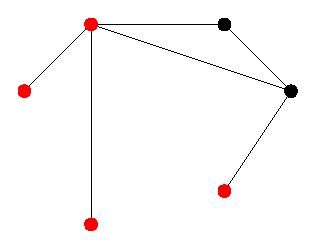
\includegraphics[width=0.35\linewidth]{graph.eps}
	\end{center}
\end{frame}
\begin{frame}{Tseitin Formulas}
	$T$-join instance $(G, T)$ as a system of linear equation.
	\pause
	\begin{itemize}[<+->]
		\item Variables correspond to edges $x_e \in \{0, 1\}$ for all $e \in E$.
		\item Define a function $\chi_{_T}: V \rightarrow \{0, 1\}, \chi_{_T}(v)=0$ iff $v
			\in T$.
		\item Let  $L_{v, \chi}$ be the equation
		$$\sum\limits_{e \in \delta(v)} x_e + \chi(v) = 0 \mod 2$$
		\item Let $\operatorname{PARITY}_{v, \chi}$ be the canonical CNF-formula
			corresponding to  $L_{v, \chi}$.
		\item For $d = \max\limits_{v \in V}\{|\delta(v)|\}$, the formula
			$\operatorname{PARITY}_{v, \chi}$ is a $d$-CNF formula with at most
			$2^{d-1}$ Clauses (why?).
		\item $T_s(G, \chi_{_T}) := \bigwedge_{v \in V} \operatorname{PARITY}_{v,
			\chi_{_T}}$, the Tseitin formula over $G$ and $T$.
	\end{itemize}
\end{frame}
\begin{frame}{Edge Expander}
	\begin{itemize}
		\item A graph $G = (V, E)$ is an $(s, \delta)$-Edge expander,
		\item[]\hspace{1cm} if $|\partial(U)| \geq \delta|U|$,  f.a. $U \subseteq V, |U| \leq s$
	\end{itemize}
	\pause
	\begin{block}{Theorem~4.3.}
		For a Tseitin Formula $T_s(G, \chi)$ over a d-regular $(s, \delta)$-edge expander
		$G$ it holds that $Sp(T_s(G, \chi)\vdash \bot) \geq \delta s / d$.
	\end{block}
	\pause
	Proof Idea:
	\begin{itemize}[<+->]
		\item Define a complexity measure.
		\item For a good choice of an expander $G$ and $T$,
		\item $T_s(G,\chi_{_T}) \vdash \bot$ contains a configuration of intermediate
			complexity.
		\item Such a configuration has a large size.
	\end{itemize}
\end{frame}

\begin{frame} \frametitle{Complexity Measure}
	We define 
	\pause
	\begin{itemize}[<+->]
		\item the complexity measure for a term $T$
		$$\nu(T) =\min\{|V'|\colon V'\subseteq V, T \land \bigwedge_{v \in V'}
			\operatorname{PARITY}_{v, \chi} \models \bot\},$$
		\item and for a configuratoin $\mathbb{C}$
		$$\mu(\mathbb{C}) =\max\{\nu(T)\colon T \models \mathbb{C}\}.$$
		\item $V^* \subseteq V$ is a {\color{red}witness} for $\nu(T)$,\\
			\hspace{1cm} if $\nu(T) = |V^*|$ and $T \land \bigwedge_{v \in
			V^*}\operatorname{PARITY}_{v, \chi} \models \bot$.
		\item A term $T^*$ is a {\color{red}witness} for $\mathbb{C}$,\\
			\hspace{1cm} if $\mu(\mathbb{C}) = \nu(T)$ and $T^* \models \mathbb{C}$.
	\end{itemize}
\end{frame}

\begin{frame}\frametitle{Intermediate complexity configuration}
	\begin{block} {Lemma~4.6}
		If $\mathbb{C} \models \mathbb{C}'$, then $\mu(\mathbb{C}) \leq \mu(\mathbb{C}')$.
	\end{block}
	(why?)\pause
	\begin{block} {Lemma~4.7}
		For a clause $A$ in $T_s(G, \chi)$ and a graph $G$ of bounded degree $d$, if
		$\mathbb{C'} = \mathbb{C} \cup A$, then $d \cdot \mu(\mathbb{C}') + 1 \geq
		\mu(\mathbb{C})$.
	\end{block}\pause
	\noindent \underline{Proof idea.} 
	\begin{itemize}
		\item Fix a witness $T^*$ for $\mu(\mathbb{C})$.
		\item Show that $\nu(T^*) \leq d\cdot \mu(\mathbb{C}') + 1$. 
		\item $\mu(\mathbb{C}') \geq \nu(T^* \land a)$ for $a \in A$.
		\item Suffices to relate $\nu(V^*)$ to $\nu(T^* \land a)$.
	\end{itemize}
\end{frame}\frametitle{Intermediate complexity configuration}

\begin{frame}
	In total we get:
	\begin{itemize}[<+->]
		\item $\mu(\emptyset) = |V|$.
		\item $\mu(\mathbb{C}) = 0,$ for $\bot \in \mathbb{C}$.
		\item $\mu(\mathbb{C}_i) \geq  \frac{1}{d} (\mu(\mathbb{C}_{i-1}) - 1)$
	\end{itemize}
	\pause
	\begin{block}{Corollary~4.8}
		For any resolution refutation $\pi$ of a Tseitin formula $T_s(G, \chi)$ over a
		connected graph $G$ of bounded degree $d$ and any positive integer $r \leq |V|$
		there exists a configuration $\mathbb{C} \in \pi$ such that the configuration
		complexity measure is bounded by $r/d \leq \mu(\mathbb{C}) \leq r$.
	\end{block}\pause
	\begin{block}{Lemma~4.9}
		Let $G$ be an $(s, \delta)$-edge expander graph. For every configuration
		$\mathbb{C}$ satisfying $\mu(\mathbb{C}) \leq s$ it holds that $Sp(\mathbb{C}) \geq
		\delta \cdot \mu(\mathbb{C})$.
	\end{block}\pause
	\noindent \underline{Proof idea.} Lower bound the size of a minimal witness $T^*$ for
	$\mu(\mathbb{C})$ (expander property).\pause It holds that $Sp(\mathbb{C}) \geq |T^*|$, since at
	most one literal per clause in $'\mathbb{C}$ is needed in the implying term.
\end{frame}

\begin{frame} \frametitle{Theorem~3.7 (restated)}
	\begin{block}{Theorem~3.7.}
		Let $F$ be a $k$-CNF formula and $\pi : F \vdash \bot$ be an $r$-DNF resolution
		refutation of $F$ in space $Sp(\pi) \leq s$. Then there exists a resolution
		refutation $\pi'$ of $F$ in width at most $W(\pi') \leq (s-2)r + k -1$.
	\end{block}
	\pause \vfill \vfill \hfill \textbf{\Large\color{NavyBlue}The end}
\end{frame}
\end{document} 
